\section{Introduction}
Definitions are explicit representations of words or phrases that are valuable
for exposing the aspects of a given term. In general, definitions are
unambiguous and succinct: they should be easy to read and understand. Recent research
has allowed the creation of neural language models that can generate useful
definitions from embeddings \cite{bosc_auto_2018, hill_learning_2016, washio_bridging_2019}. Word embeddings are vector representations of words that have been employed in a variety of \textit{natural language
    processing} (NLP) tasks. They are useful for capturing lexical syntax and
semantic similarity. Mikolov et al. \cite{mikolov_distributed_2013} have shown that
basic mathematical operations applied to word embeddings can have meaningful
language understanding. However, as continuous representations, the
interpretability of word embeddings is limited.

\begin{figure}[h]
    \centering
    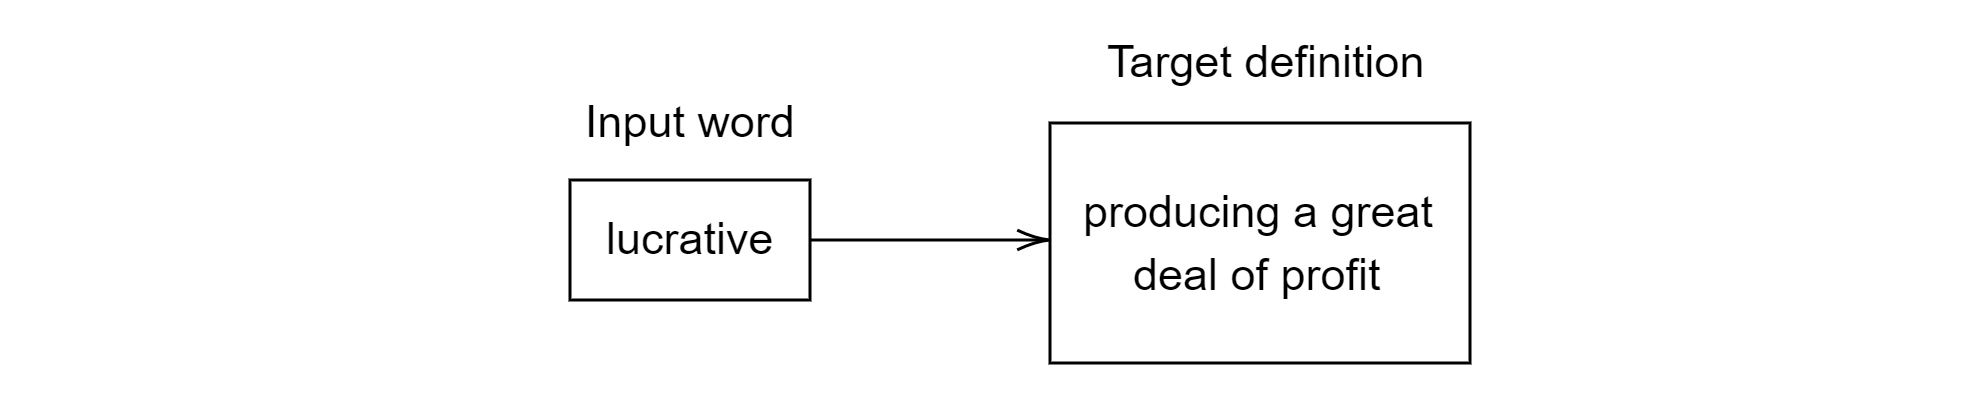
\includegraphics[width=.9\textwidth]{assets/figures/monoseme.png}
    \caption{Monoseme example word and definition. A definition model could
        generate the definition \textit{producing a great deal of profit} for the
        input word \textit{lucrative}.}
    \label{fig:monoseme}
\end{figure}

The problem of \textit{definition modeling} was proposed by Noraset et al.~\cite{noraset_definition_2016} to evaluate word embeddings. The task of definition modeling is to generate a definition for a given term. The goal of a model trained on this task is to train on word embedding and definition pairs to learn to generate a definition for a given word or phrase. An example of a \textit{monoseme} (word with a single definition) is given in Figure~\ref{fig:monoseme}. Given the input word \textit{lucrative}, a model trained on
the task of definition modeling would produce the output definition
\textit{producing a great deal of profit}.

\begin{figure}[h]
    \centering
    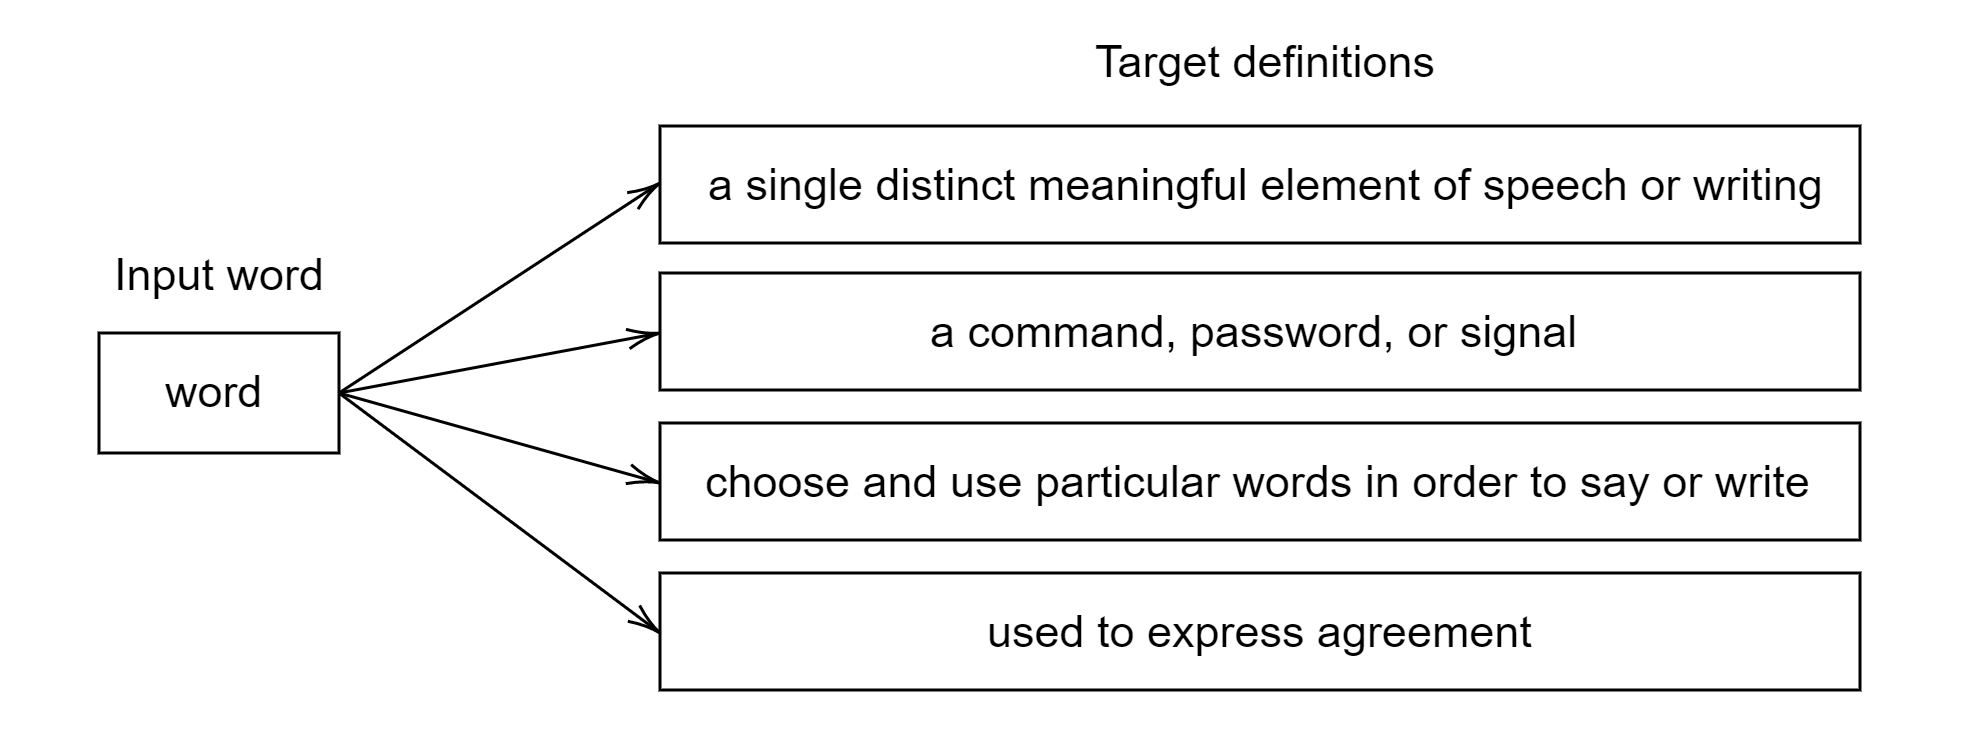
\includegraphics[width=.9\textwidth]{assets/figures/polyseme.png}
    \caption{Polyseme example word and definition. A definition model could generate any of the target definitions.}
    \label{fig:polyseme}
\end{figure}

In addition to being a relatively new language modeling task, definition
modeling has attracted attention from the literature in a number of areas.
First, it was shown that the definition model has poor performance when
generating definitions for polysemes: words with multiple definitions
\cite{gadetsky_conditional_2018}. An example polysemous word is shown in Figure
\ref{fig:polyseme}. Given the input \textit{word}, the goal of a definition
model would be to generate one of the target definitions, most ideally the
closest definition to the word sense of the input. However, it is challenging to
know the word sense given only the input word.

The problem of polysemous words was not addressed in the original work, as only one definition mapped to each word. Once researchers attempted to address this problem, they found that the definition model could not learn the semantics of the polyseme with only the word as an input. Therefore, it was necessary to augment the definition model with additional information, namely, an example sentence that sets the word to be defined (\textit{definiendum}) inside to
provide context. This method has been shown to alleviate the problem of generating definitions for polysemes and also improve the performance of the definition model on several measures~\cite{bevilacqua_generationary_2020,
    gadetsky_conditional_2018, mickus_mark_2019}.

\begin{figure}[h]
    \centering
    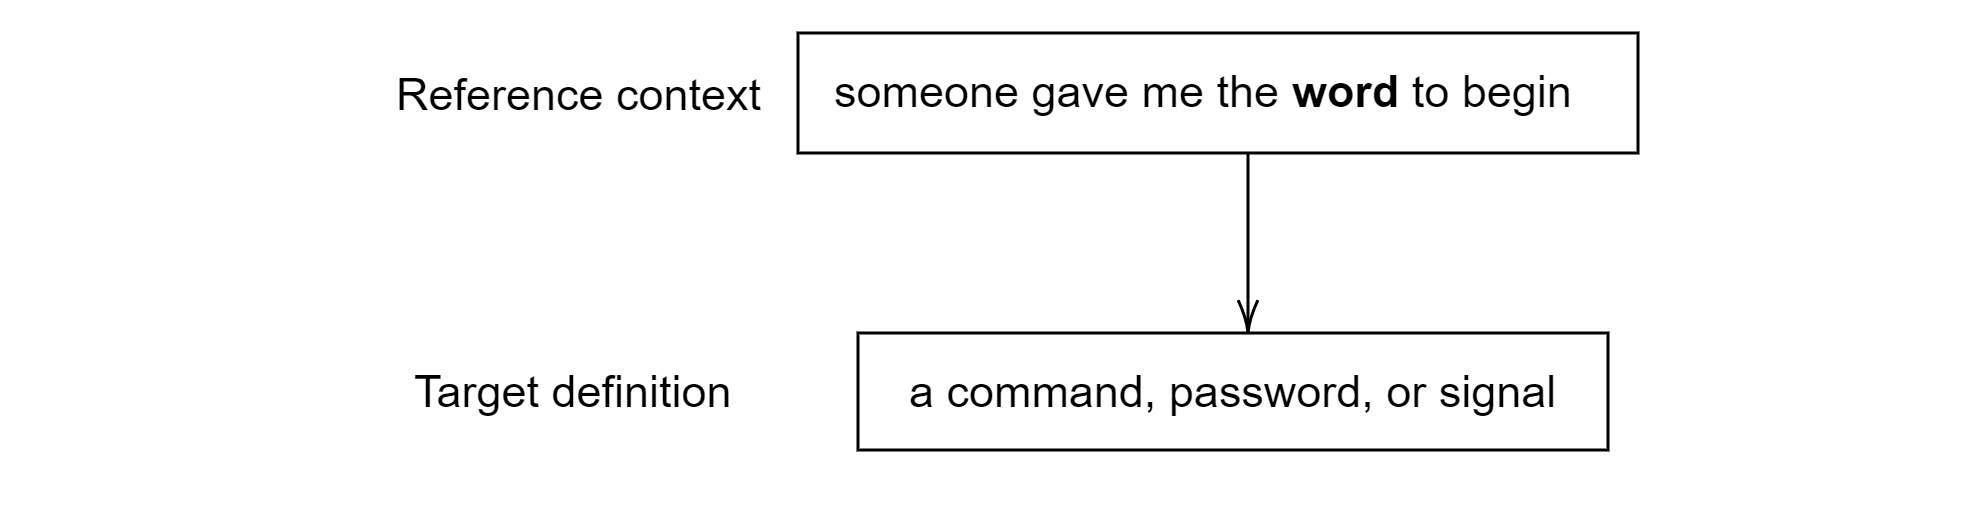
\includegraphics[width=.9\textwidth]{assets/figures/context.png}
    \caption{Context-dependent definition task. The word to be defined is marked
        in bold. In this case, although \textbf{word} is a polyseme, there is only
        one correct target definition due to the contextual information provided.}
    \label{fig:context_poly}
\end{figure}

Definition modeling, especially as a sequence-to-sequence task, is similar to other NLP tasks, such as \textit{word-sense disambiguation}, \textit{word-in-context}, and \textit{definition extraction}~\cite{bevilacqua_generationary_2020, huang_cdm_2021}. When using context to generate a definition from an input word, the input's word sense must be extracted to select the correct definition. The goal of word-sense disambiguation is similar in that the goal of word-sense disambiguation is to identify the sense of a word used in a sentence. Similarly, definition extraction seeks to extract definitions of terms from an existing corpus~\cite{huang_cdm_2021}. Figure~\ref{fig:context_poly} shows an example of definition modeling in a context-dependent situation. In the example, a reference context is given. Inside the reference context, a target word
\textit{word} is marked as the word to be defined. The goal of a definition model given this context and marked word would be to generate the target definition \textit{a command, password, or signal}.

Our paper is organized into three sections. Section 2 reviews definition modeling methods as well as word embeddings. Section 3 shares benchmark datasets
and statistics that can be used when formulating and evaluating a definition modeling method. Section 4 explores challenges encountered in this research field and gives suggestions for future work.
